\documentclass[11pt]{article}
\usepackage[a4paper,margin=0.65in]{geometry}
\usepackage[T1]{fontenc}
\usepackage{lmodern}
\usepackage{tikz}
\usetikzlibrary{arrows.meta,positioning,shapes.geometric,fit,calc}
\usepackage{pdflscape}
\usepackage{float}
\usepackage{caption}
\pagestyle{plain}
\setlength{\parindent}{0pt}

\tikzset{
  classbox/.style={draw, rounded corners=2pt, fill=blue!3, align=left,
    font=\small, inner sep=5pt, text width=5.0cm},
  smallclass/.style={draw, rounded corners=2pt, fill=blue!3, align=left,
    font=\small, inner sep=5pt, text width=4.2cm},
  module/.style={draw, rounded corners=3pt, fill=teal!7, align=center,
    minimum height=9mm, text width=3.4cm, font=\small},
  datastore/.style={draw, cylinder, shape border rotate=90, aspect=0.25,
    fill=orange!10, align=center, minimum height=9mm, text width=2.8cm, font=\small},
  decision/.style={diamond, draw, fill=yellow!12, align=center, aspect=2.0,
    inner sep=2pt, font=\small},
  flow/.style={-{Stealth[length=2.2mm]}, thick},
  dependency/.style={-{Stealth[length=2mm]}, dashed, thick},
  association/.style={-{Stealth[length=2mm]}, thick}
}
\begin{document}
\begin{center}
{\LARGE\bfseries Automated Plagiarism Checker}\\[2mm]
{\large PlagiarismReport UML Class Diagram}
\end{center}
\vspace{4mm}

\begin{figure}[H]\centering
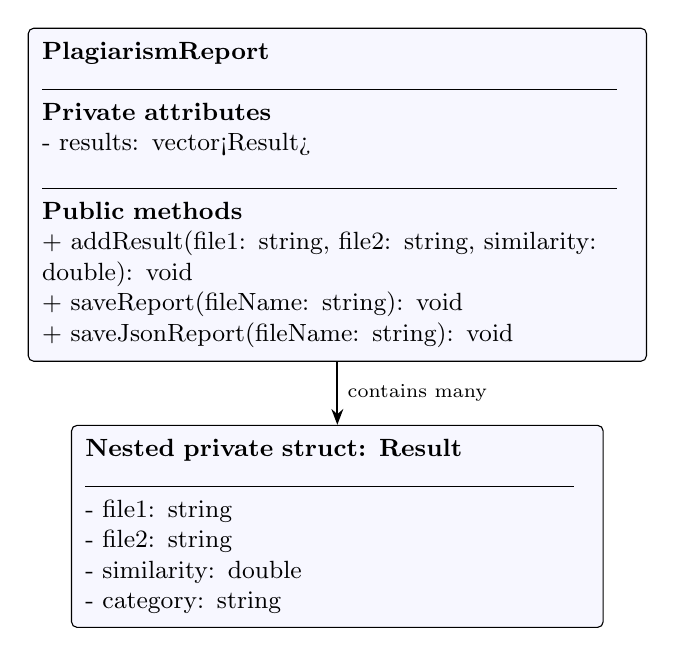
\begin{tikzpicture}[node distance=8mm]
\node[classbox,text width=7.5cm] (p) {
\textbf{PlagiarismReport}\\\rule{7.3cm}{0.4pt}\\
\textbf{Private attributes}\\
- results: vector<Result>\\[1mm]\rule{7.3cm}{0.4pt}\\
\textbf{Public methods}\\
+ addResult(file1: string, file2: string, similarity: double): void\\
+ saveReport(fileName: string): void\\
+ saveJsonReport(fileName: string): void
};
\node[classbox,text width=6.4cm,below=of p] (r) {
\textbf{Nested private struct: Result}\\\rule{6.2cm}{0.4pt}\\
- file1: string\\
- file2: string\\
- similarity: double\\
- category: string
};
\draw[association] (p.south) -- node[right,font=\scriptsize]{contains many} (r.north);
\end{tikzpicture}
\caption{UML class diagram for PlagiarismReport.}
\end{figure}

\end{document}
